\newpage
% Définir ce qu'est un logiciel vidéo non linéaire, non intruisif,
% Ses fonctionnilités basique,
% Définir le term de logiciel libre
%
\section{Introduction}
    \paragraph{}
        Nowadays we are seeing more and more free and open source projects
        getting pretty popular and used worldwide. This is true in many
        domains where computer science is influential. But there are
        still lots of computer science domains where FOSS are actually not that
        popular.

    \paragraph{}
        This document concentrate on this subject in the world of video
        edition, and particularly (but not only) the use of libre softwares
        for professional video edition.

    \paragraph{}
        Not that the number of initiatives aiming at creating a FOSS video
        editor is small, as the following diagram shows:

        \begin{figure}[!htbp]
            \begin{center}
                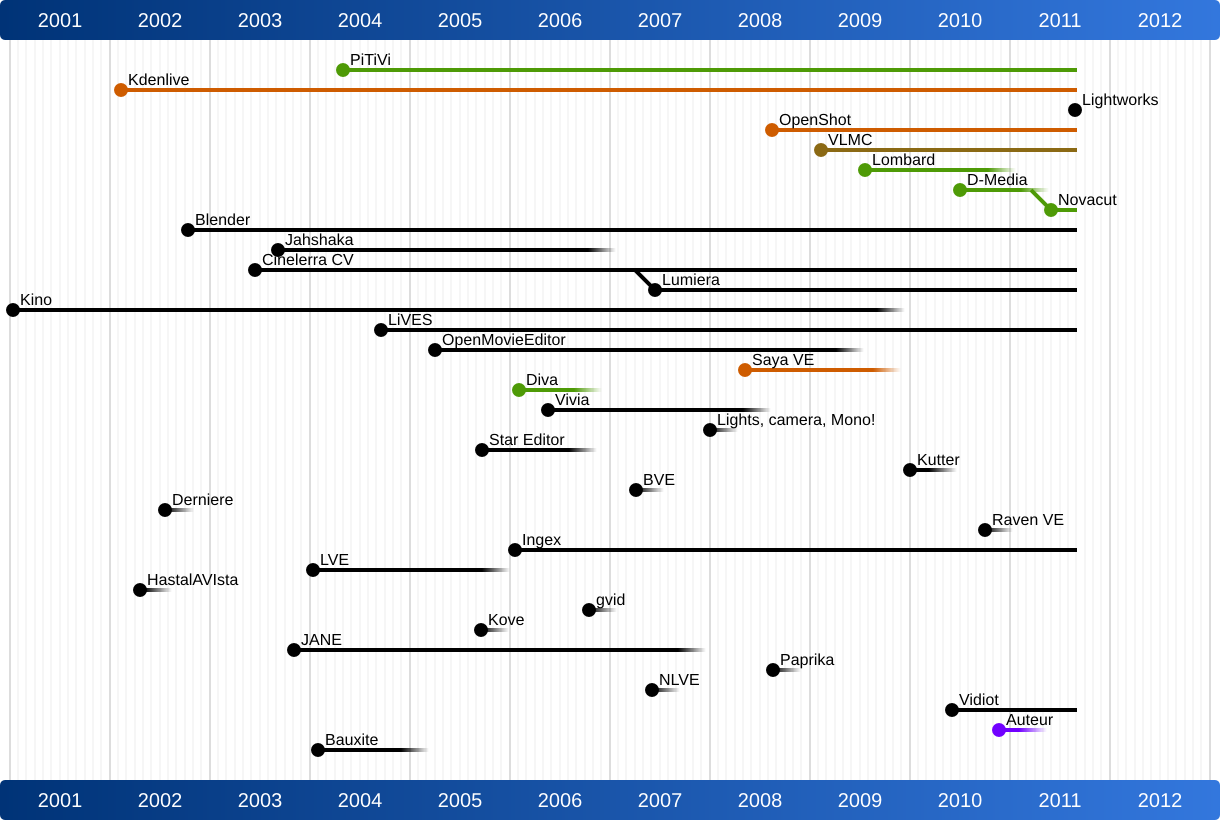
\includegraphics[width=0.9\textwidth]{images/open-source-video-editor-timeline}
            \end{center}
            \caption{Open source video editor timeline}
            \label{Yes}
        \end{figure}

    \paragraph{}
        But all projects don't have the same goal, most of them are
        done for people to edit little family, humanistic\ldots videos,
        and don't actually have a professional focus. Moreover, most of the
        projects are not really active, and do not have any company pushing them
        in order to be introduced to professionals.

        This document will not focus too much on this category of software, but
        actually on those which have an ambition to be more than ``toy''
        softwares. (As I am still starting to write this thesis, I can not define
        precisely what are those softwares, and this is a task I have to
        concentrate on soon.)


    \subsection{Picture of the video edition world}
        \paragraph{}
            As the goal is to draw a picture of the whole video editor world, I
            will start describing it this way:
            \begin {itemize}
                \item {New platforms on which video editor are emerging:}
                \begin {itemize}
                    \item {Smartphone: Android, Meego, iphone}
                    \item {Tablet PC: Android, Meego, iphone}
                    \item {\ldots}
                \end {itemize}
                \item {Enthusiast video content creators}
                \item {Professional video content creators}
                \begin {itemize}
                    \item {Video clip producers}
                    \item {Short movie producers}
                    \item {Television content creators}
                    \item {Blockbuster producers (also think 3D support)}
                    \item {Art house movie creators}
                \end {itemize}
            \end {itemize}

    \subsection{Focus on professional video editors}
        \paragraph{}
            After describing the video edition world, and how it is currently
            evolving, I will focus on the main video editing usage this documents
            aims at analyzing: ``Video editors for Professional video content
            creators''. Se concentrer sur dreamworks \cite{RobinRowe2001}

       \subparagraph{}
            To do so, the first thing is to define what professional means. I will
            also concentrate on what these people expect from a video editing tool.
            What are the main feature they need, and this should also be done
            making sure to distinguish the different kind of professional video
            editor that exist. I will also define to what extent stability of the
            tool is important. In this part I will get started by introducing
            Interviews from people working in this domain, being sure to get an
            as large as possible point of view.

    \subsection{State of the art}
       \paragraph{}
            This is where I will concentrate on drawing the State of the art in
            the open source world. This is a  technical report of the existing
            solutions.  The idea is to investigate existing technologies and
            check what use cases those technologies can fulfill, and what they
            can not. I will also see what are the plans of the developers of
            those technologies, make an analysis of the communities, and see
            how much support they have from companies. In this part, I will of
            course also analyze the video editors using those technologies and
            their communities. The analysis of communities, the way they work,
            their efficiency should be an important point of this part.

    \subsection{Focus on commercial solutions}
       \paragraph{}
            Right after analyzing the state of open source solutions and
            technologies, I will concentrate on what is going on in the commercial
            world. I will make an analysis of the main solutions, see how they
            fill the different needs this document describes. I will analyze the
            market and see if there is a real need for other solutions to come
            up, and what we should expect from them.

    \subsection{Comparison of the two worlds}
        \paragraph {}
            Now that I have a description of the two world, I will have to compare
            them, focusing on the topic I want to tackle: professional video
            editors. This comparison should take into consideration what I got from
            the interviews. This should be technical when possible, but very user
            oriented, which means that the user-friendliness of the solutions should have
            been described, and will be taken into account.

    \subsection{Open source lacks}
        \paragraph{}
            I will then analyze the lacks open source solutions suffer from,
            and discuss the ways to get it solved. In this part, I will analyze
            the solutions that could be found to get more people involved in
            communities, users, as well as developers, and how companies could get
            money from it.

    \paragraph{At the end of this document,} you should have a good
        overview of the video editing world, understand what FOSS can offer to
        professionals in this domain. You should also understand what is the
        current state of libre softwares is now, where they are going, and how
        the communities are driving those projects.
